\documentclass[12pt,letterpaper]{article}


\newcommand{\studentname}{Ben Bassett}

\title{\textsc{Lab 10: Diffraction of Pet Hair}}
\newcommand{\shorttitle}{Diffraction of Pet Hair}

\newcommand{\course}{PHY310}
\newcommand{\labdate}{11-12-2024}

%------------------------------------------------------------------------------------------------------------

\usepackage[letterpaper,left=1in,right=1in,bottom=1in,top=1in]{geometry}
\usepackage{fancyhdr}
\usepackage{subfigure}
\usepackage{graphicx}
\usepackage{amsmath}
\DeclareMathOperator{\sinc}{sinc}
\usepackage{cleveref}
\usepackage{booktabs}
\usepackage[british]{babel}
\usepackage[square,comma,numbers,sort&compress]{natbib}
\usepackage{csvsimple}
\usepackage{graphicx}
\usepackage{pgfplotstable}
\usepackage{textcomp,gensymb}
\usepackage{array}
\usepackage{tabu}
\usepackage{multirow}
\usepackage{url}
\usepackage{lipsum}
\usepackage{dsfont}
\pgfplotsset{compat=1.9}% supress warning
\begin{document}

%------------------------------------------------------------------------------------------------------------

\setlength{\parindent}{1em}
\setlength{\parskip}{0.5em}
\author{\course~Lab Journal \\ \\ \studentname} % \,\& \labpartner}
\date{\labdate}

\renewcommand\abstractname{Summary}

\pagestyle{fancy}
\fancyhead{}
\fancyhead[l]{\course:~\shorttitle}
\fancyhead[r]{\studentname}
\fancyfoot{}
\fancyfoot[C]{\thepage}
\renewcommand{\headrulewidth}{0pt}
\renewcommand{\footrulewidth}{0pt}

\renewcommand\bibname{References}

%------------------------------------------------------------------------------------------------------------

\renewcommand\abstractname{Abstract}
\maketitle

% COMMENT IN IF ASKED TO SUBMIT REPORT WITH ABSTRACT
\begin{abstract}
In this experiment we set out to measure the diameter of pet hair using the far-field approximation for diffraction patterns at different distances from a diffracted laser.
\end{abstract}

\section{Experimental Apparatus}

Materials given were an optics track, 650 nm laser diode, pet hair, a ruler, and a screen. Our setup is illustrated in Figure \ref{fig:setup}.

\begin{figure}[h]
    \centering
    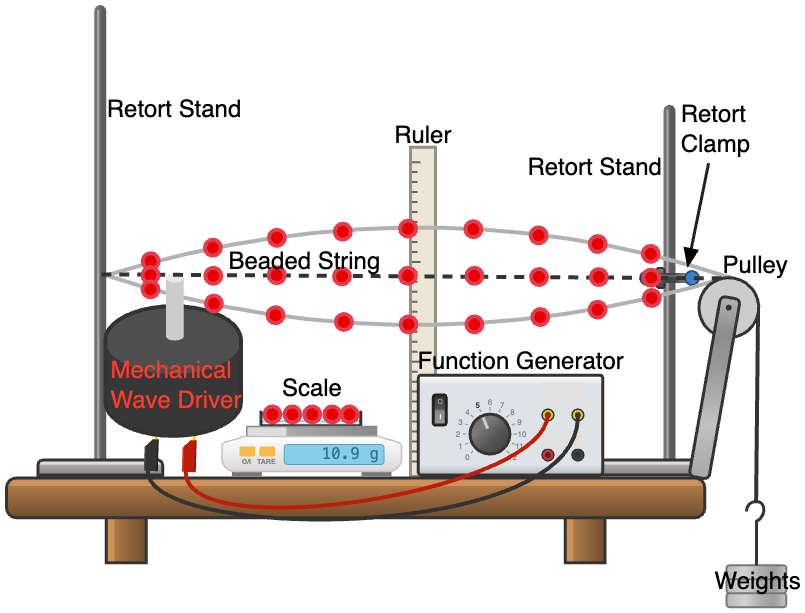
\includegraphics[width=6in]{images/setup.png}
    \caption{The final optics track setup}
    \label{fig:setup}
\end{figure}

% \pagebreak
\section{Procedure}

We setup the optics track such that the laser was a 110 cm and the hair was at 100 cm, then we started the screen 10 cm away from the hair, and incremented up by 10 cm until we reached one hundred. Each increment we photographed the diffraction pattern next to a laser (See Figure 2) and determined the width of the center constructive interference pattern.

\begin{figure}[h]
    \centering
    \includegraphics[width=6in]{images/diffraction.jpg}
    \caption{Photograph of the diffracted laser 20 cm from the hair}
    \label{fig:setup}
\end{figure}

\section{Results}

\begin{table}[h]
\centering
\begin{tabular}{|c|c|c|c|}
\hline
Distance (cm) & Beam Width (mm) & Diameter (mm) \\
\hline
10.0 ± 0.1 & 2.5 ± 0.3 & 0.052 ± 0.006 \\
20.0 ± 0.1 & 3.0 ± 0.3 & 0.087 ± 0.009 \\
30.0 ± 0.1 & 3.5 ± 0.3 & 0.111 ± 0.010 \\
40.0 ± 0.1 & 4.0 ± 0.3 & 0.130 ± 0.010 \\
50.0 ± 0.1 & 5.0 ± 0.3 & 0.130 ± 0.008 \\
60.0 ± 0.1 & 6.5 ± 0.3 & 0.120 ± 0.006 \\
70.0 ± 0.1 & 8.0 ± 0.3 & 0.114 ± 0.004 \\
80.0 ± 0.1 & 9.5 ± 0.3 & 0.109 ± 0.003 \\
90.0 ± 0.1 & 11.5 ± 0.3 & 0.102 ± 0.003 \\
100.0 ± 0.1 & 13.0 ± 0.3 & 0.100 ± 0.002 \\
\hline
\multicolumn{2}{|c|}{Average of 30-100 cm} & 0.115 ± 0.002 \\
\hline
\end{tabular}
\caption{Beam width measurements and calculated diameters}
\label{tab:beam_measurements}
\end{table}

We compute the diameter of the hair using our knowledge of diffraction patterns: there is constructive interference at 

\begin{equation}
    d\sin(\theta)=n\lambda
\end{equation}

Where $d$ is the diameter of the hair and $\lambda$ the wavelength of the laser, which in our case was 650 nm.

Since we only took data from the first constructive pattern, $n=1$. Since our angle $\theta$ is quite small, we can use our small angle approximations to say

\begin{equation}
    \sin\theta\approx\tan\theta=\frac{w}{2L}
\end{equation}

where $w$ is the width of $n=1$ constructive pattern, and $L$ is the distance between the hair and the screen. Let's use this to construct our final diffraction condition

\begin{align}
    d\left(\frac{w}{2L}\right) &= \lambda \\
    d&=\frac{2\lambda L}{w}
\end{align}

This is the final relationship I used to compute the diameter of the hair in Table 1. Graphing the data in Figure 3, it seems that the far-field approximation we use in Equation 1 breaks down about 20 cm from the hair.

\begin{figure}[h]
    \centering
    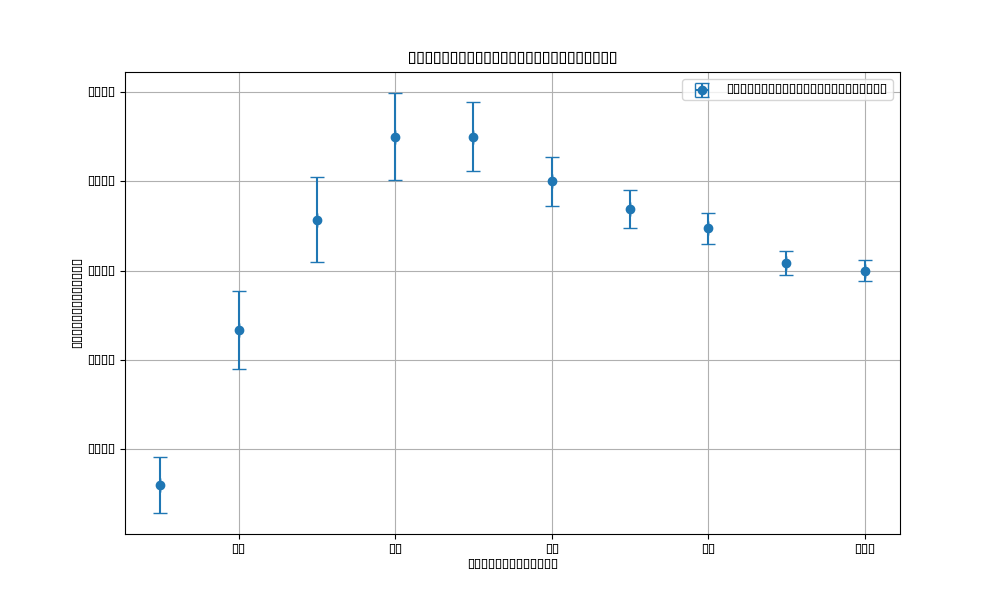
\includegraphics[width=7in]{images/beam_diameter.png}
    \caption{Graph of the computed diameters with distance}
    \label{fig:setup}
\end{figure}

 If we only use the last 8 data points, our average diameter is $\mathbf{0.115 \pm 0.002} \textbf{ mm}$.

\section{Conclusions}

We used the far-field approximation to successfully measure the diameter of the dog hair at $\mathbf{0.115 \pm 0.002} \textbf{ mm}$, a reasonable number!

% \bibliographystyle{unsrtnat}
% \bibliography{references}

\end{document}
